



%%CHAP. Theory

\begin{figure}[h]
\centering
  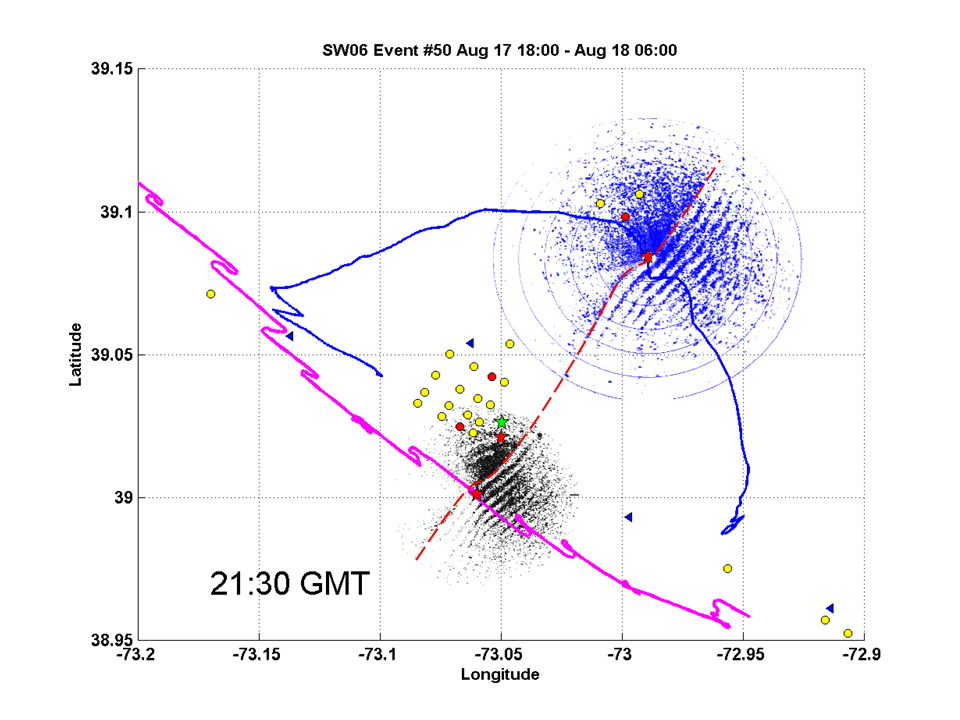
\includegraphics[width=0.8\textwidth]{IW_radar2.png}\\
  \caption{Radar image of internal wave surface signature at 21:30GMT . }
  \label{fig:IW_radar2}
\end{figure}

\begin{figure}[h]
\centering
  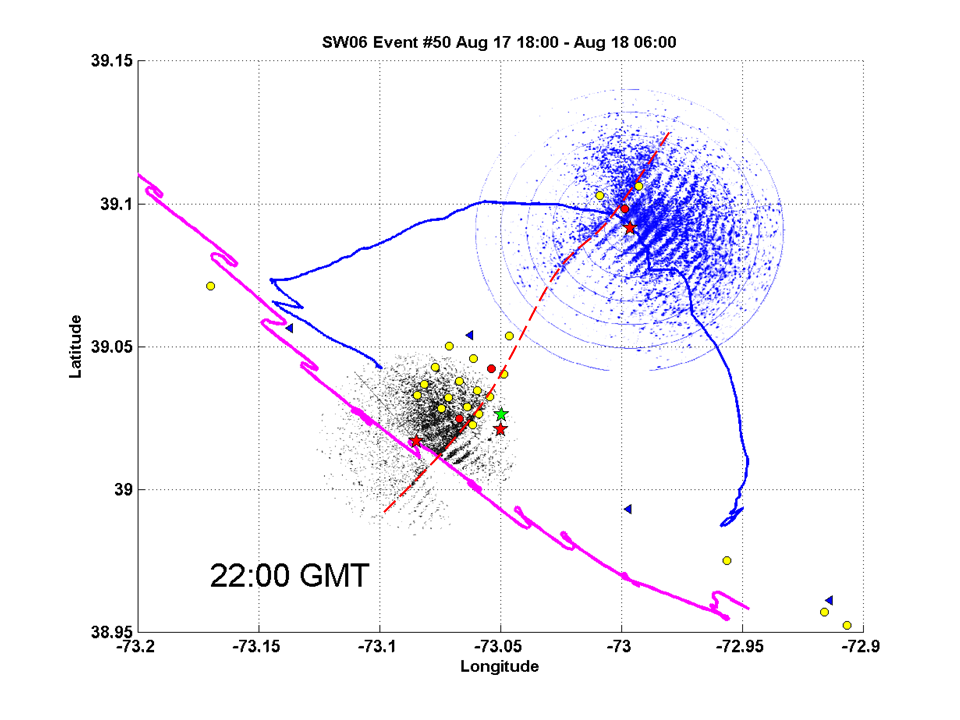
\includegraphics[width=0.8\textwidth]{IW_radar1.png}\\
  \caption{Radar image of internal wave surface signature at 22:00GMT . }
  \label{fig:IW_radar1}
\end{figure}

% \begin{figure}[h]
%\centering
 % 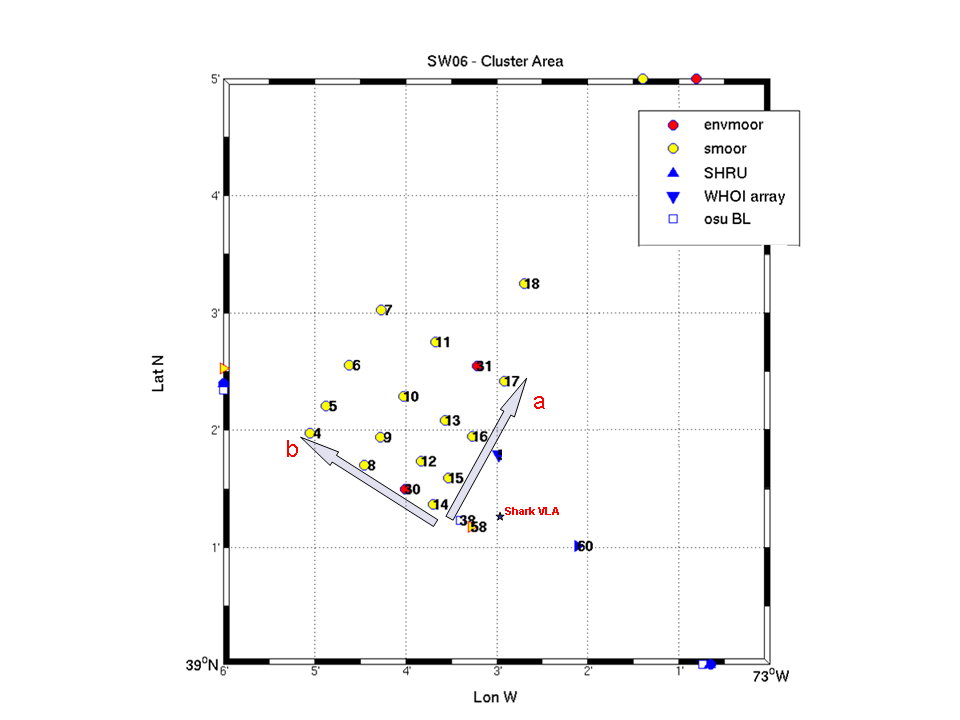
\includegraphics[width=0.8\textwidth]{T_farm2.png}\\
 % \caption{Thermistor farm deployed in SW06. Edge (a) \& (b) are parallel and perpendicular to the internal wave fronts, respectively. }
  %\label{fig:tfarm}
%\end{figure}

 \begin{figure}[h]
\centering
  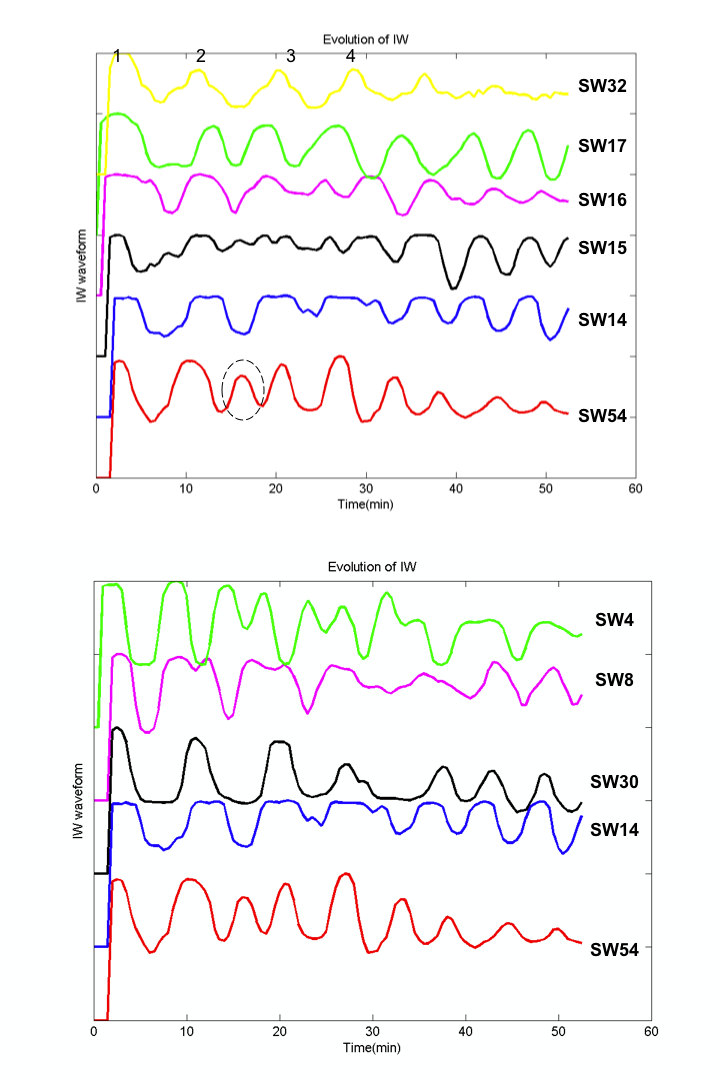
\includegraphics[width=0.8\textwidth]{tfarm_iw.png}\\
  \caption{Temperature data recorded by the thermistor farm during SW06 event 50. }
  \label{fig:tfarm_dir}
\end{figure}

\begin{figure}[h]
\centering
  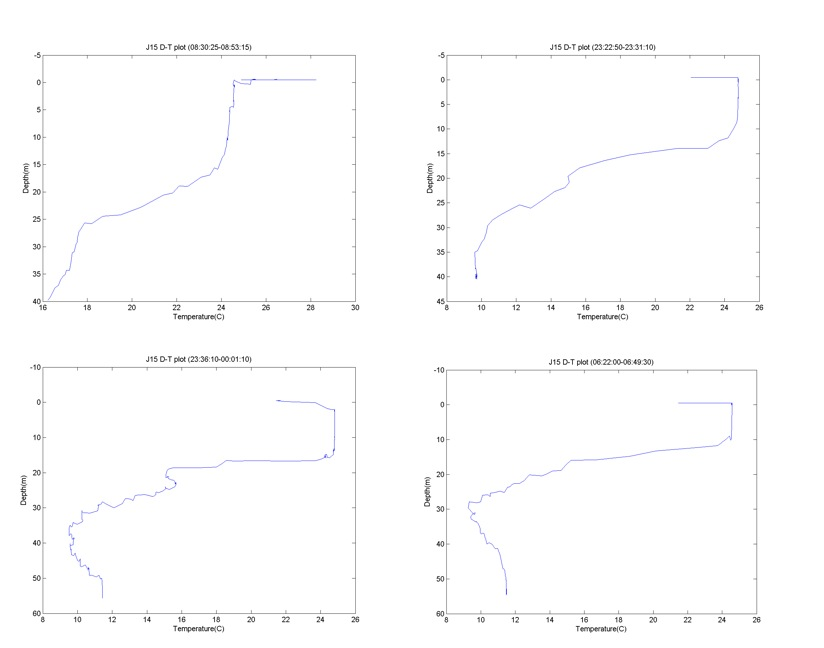
\includegraphics[width=0.8\textwidth]{water_temp4.jpg}\\
  \caption{Temperature profile recorded by TD sensor attached to J15 transducer}
  \label{fig:water_temp4}
\end{figure}

%\begin{figure}[h]
%\centering
  %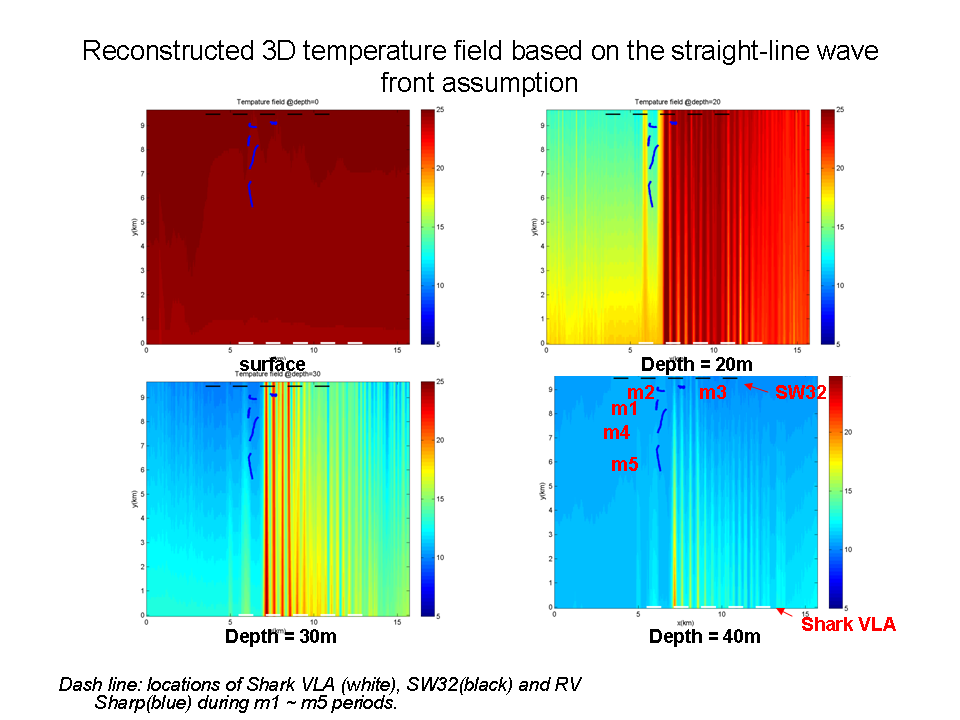
\includegraphics[width=0.8\textwidth]{3D_temp_recon.png}\\
  %\caption{Reconstructed temperature field and the movement of source and receiver in the internal wave coordinates}
  %\label{fig:water_temp4}
%\end{figure}

\begin{figure}[h]
\centering
  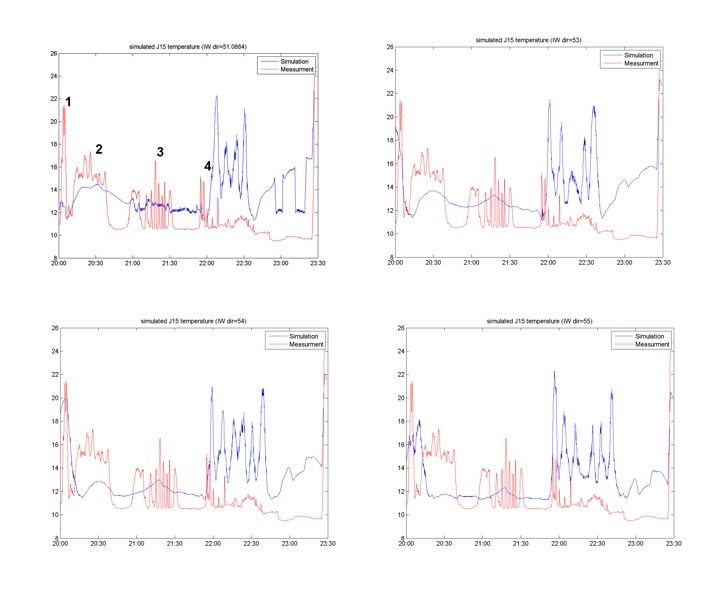
\includegraphics[width=0.8\textwidth]{J15_sim.jpg}\\
  \caption{Simulated J15 recored in reconstructed 3D environment}
  \label{fig:water_temp4}
\end{figure}

%\begin{figure}[h]
%\centering
  %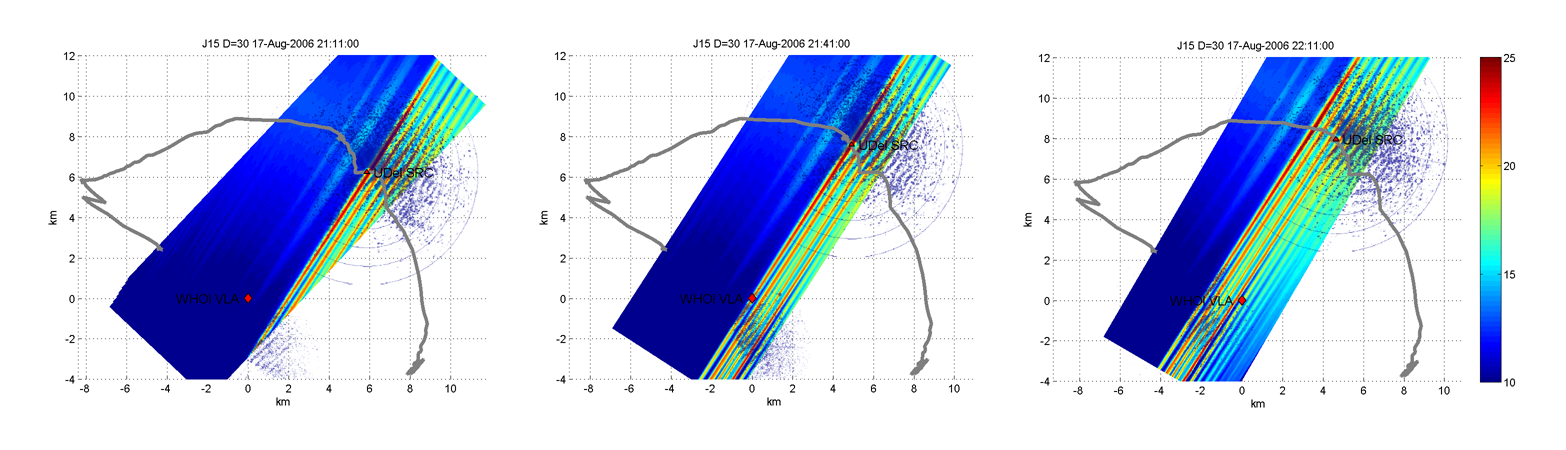
\includegraphics[width=\textwidth]{3D_interp_radar.png}\\
  %\caption{Reconstructed temperature field (depth = 30m) with radar image overlay at GMT21:11, 21:41 \& 22:11, Aug 17th.}
  %\label{fig: 3D_interp_radar}
%\end{figure}




\clearpage

\begin{figure}[H]
\centering
  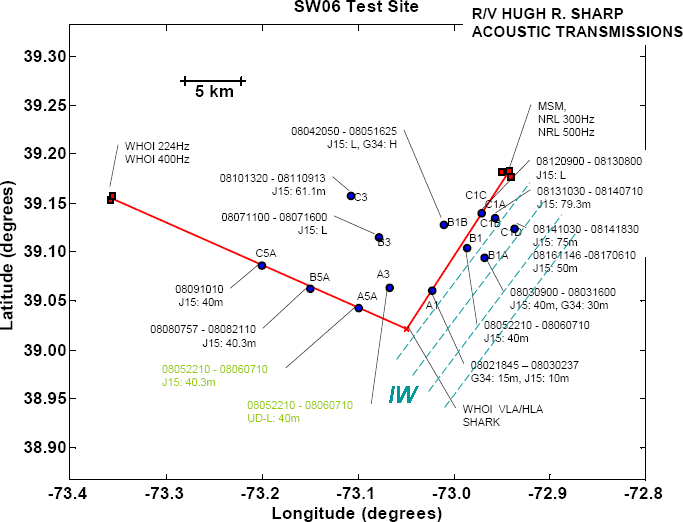
\includegraphics[width=\textwidth]{transmission1.png}
  \caption{Positions of the J15 acoustic source deployed from R/V Sharp during SW06 experiment. Some positions were chosen to vary the angle between the acoustic track and the IW propagation.}
  \label{fig:transmission}
\end{figure}


\begin{figure}[H]
  \centering
  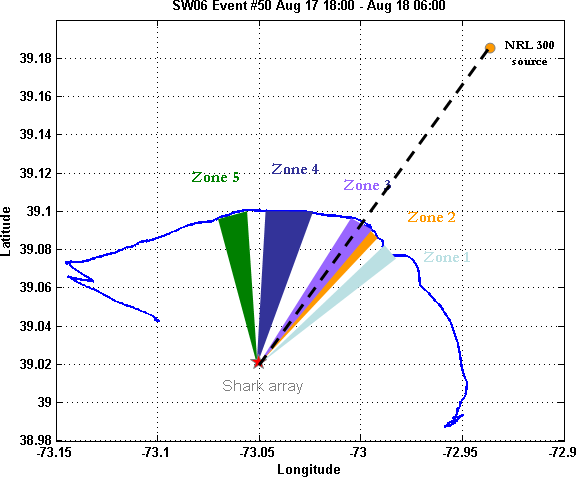
\includegraphics[width=\textwidth]{zones.png}
  \caption{Positions of the fixed and mobile acoustic sources.}\label{fig:zones}
\end{figure}


\begin{figure}[H]
\centering
  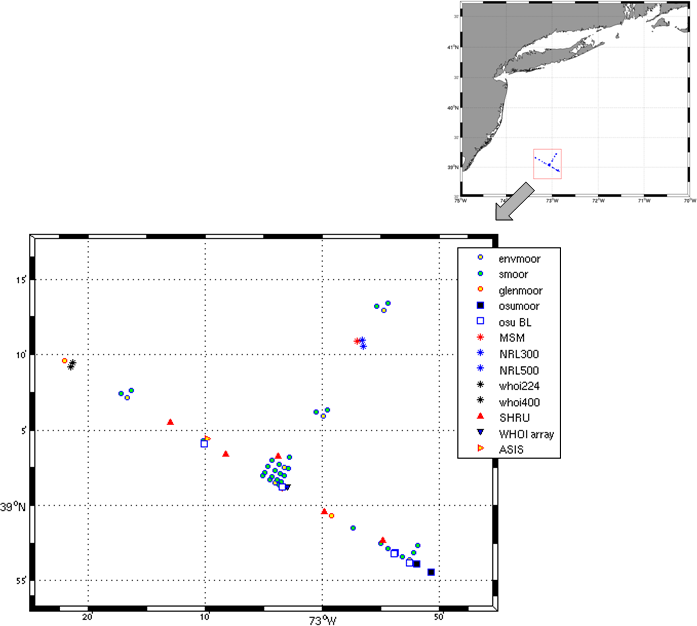
\includegraphics[width=\textwidth]{moorings_site.png}\\
  \caption{SW06 mooring locations}
  \label{fig:moorings}
\end{figure}



\begin{figure}[H]
\centering
  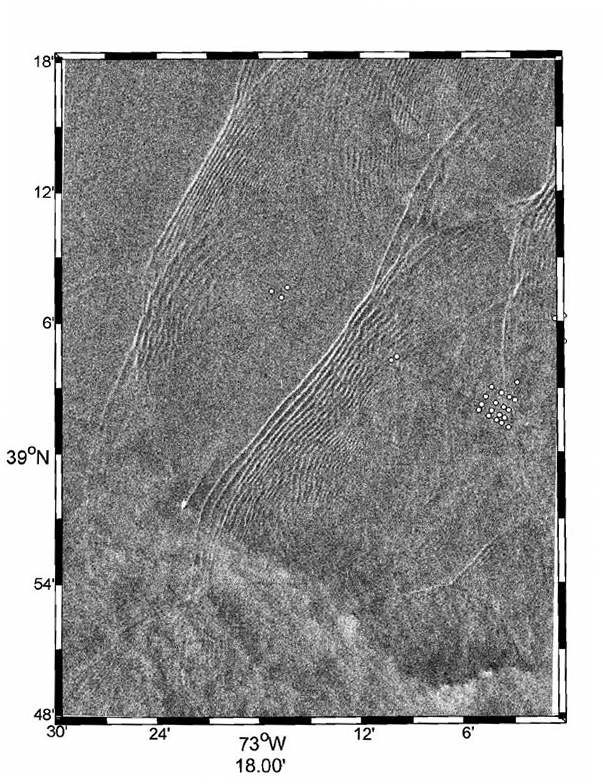
\includegraphics[width=\textwidth]{satellite.png}\\
  \caption{Radarsat observation from August 13, 2006. Some of the SW06
moorings are shown in the figure to provide scale.}
  \label{fig:satellite}
\end{figure}


\begin{figure}[H]
\centering
  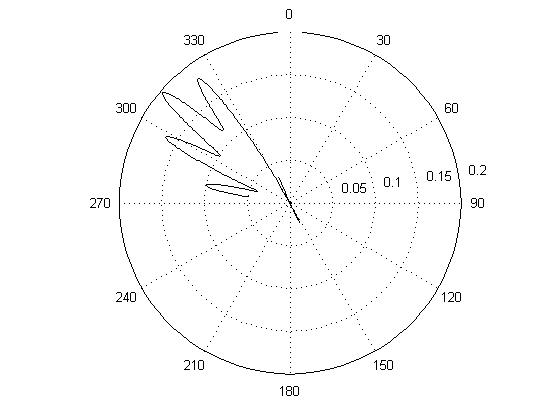
\includegraphics[width=\textwidth]{iw_direction.jpg}\\
  \caption{Calculated direction of dominant IW event observed based on 60 observed IW events}
  \label{fig:IW_dir}
\end{figure}

\begin{figure}
  \centering
  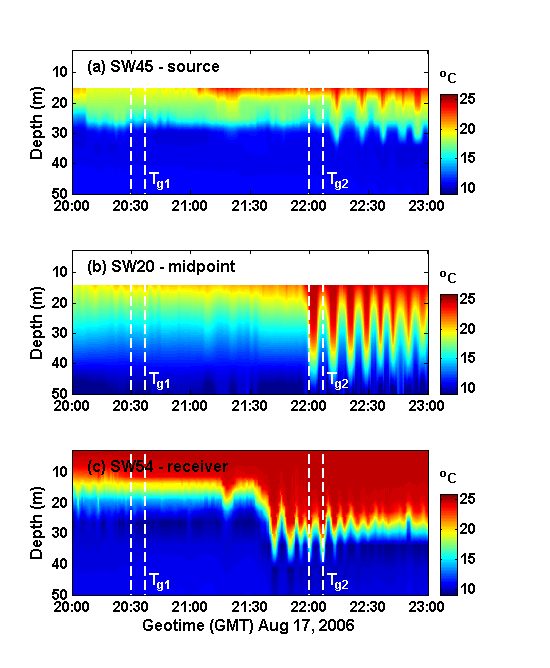
\includegraphics[width=\textwidth]{jasa2_temperature.png}
  \caption{Temperature profiles measured at (a) the acoustic source, (b) the midpoint between the source and receiver, and (c) at the Shark WVHLA during internal wave Event 50, August 17, 2006 from 20:00 to 23:00 GMT. $T_{g1}$ = 20:30 to 20:37 GMT and $T_{g2}$ = 22:00 to 22:07 GMT.}\label{fig:temp}
\end{figure}

%%--F1
\begin{figure}[H]
  \centering
  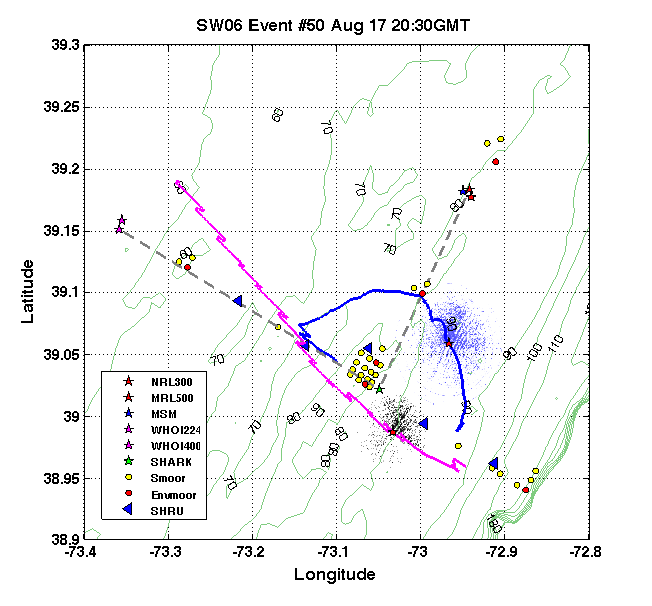
\includegraphics[width=\textwidth]{Aug17_2030_t.png}
  \caption{Surface expression of internal wave package at 20:30GMT, Aug. 17, recorded by R/V Sharp and R/V Oceanus. Blue and red lines indicate their movements, respectively. (Blue: R/V Sharp's, red: R/V Oceanus'}\label{fig:r2130_r}
\end{figure}

\begin{figure}[H]
  \centering
  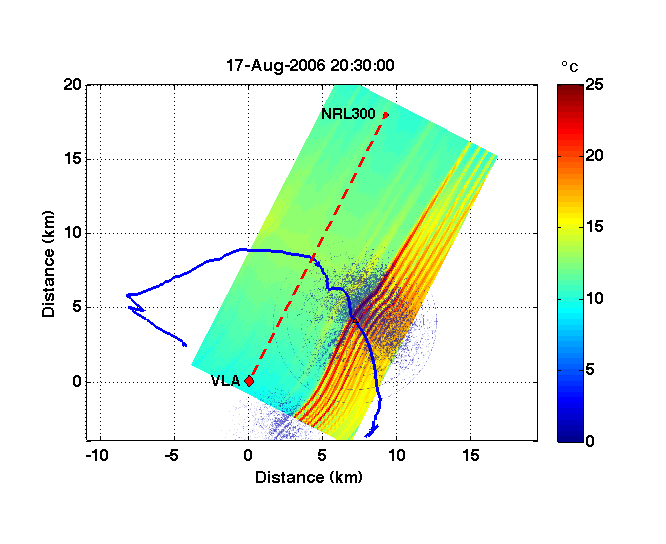
\includegraphics[width=\textwidth]{sw06_Tempr_Depth30m_2006Aug17_203000_radar_curve_thesis1.png}
  \caption{Interpolated internal wave field at 20:30GMT, Aug. 17, water depth = 20m. (Refer to section 3.4 for detailed interpolation method)}\label{fig:r2130_i}
\end{figure}

\begin{figure}[H]
  \centering
  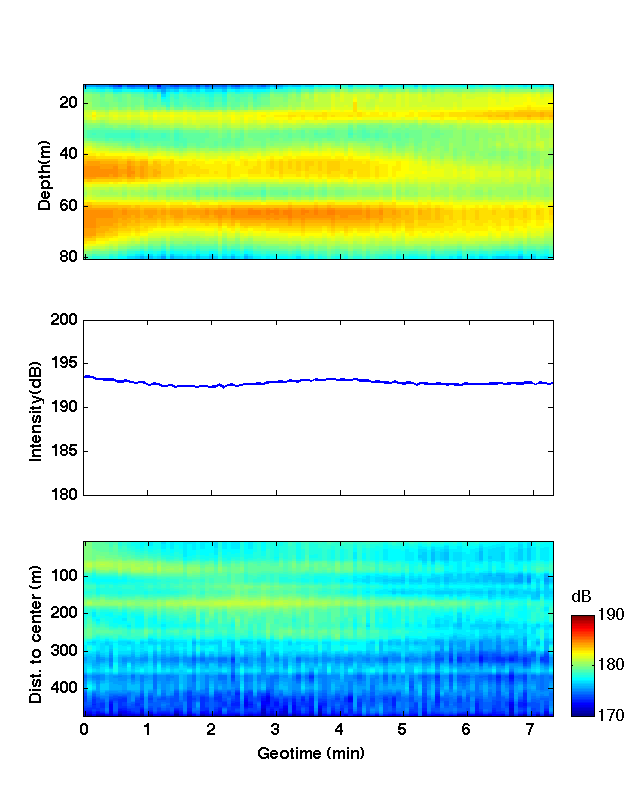
\includegraphics[width=\textwidth]{nrl300_060817T2030_vla_hla_intens_geotime2.png}
  \caption{Received signal on Shark VLA (top), HLA (bottom) and signal intensity (middle) from Aug.17 20:30GMT to 20:37GMT }\label{fig:a2130}
\end{figure}

\begin{figure}[H]
  \centering
  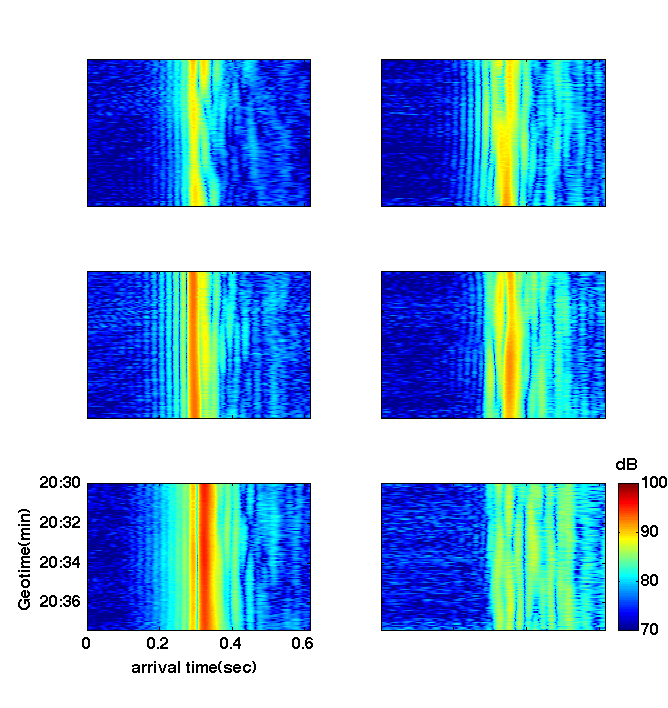
\includegraphics[width=\textwidth]{sw06_broadband_mf_nrl300_F1_6in1_thesis.png}
  \caption{Mode decomposition of received signal on Shark VLA. 
    Left column: mode 1-3, right column: mode 4-6 }\label{fig:m2130}
\end{figure}



%%--F2
\begin{figure}[H]
  \centering
  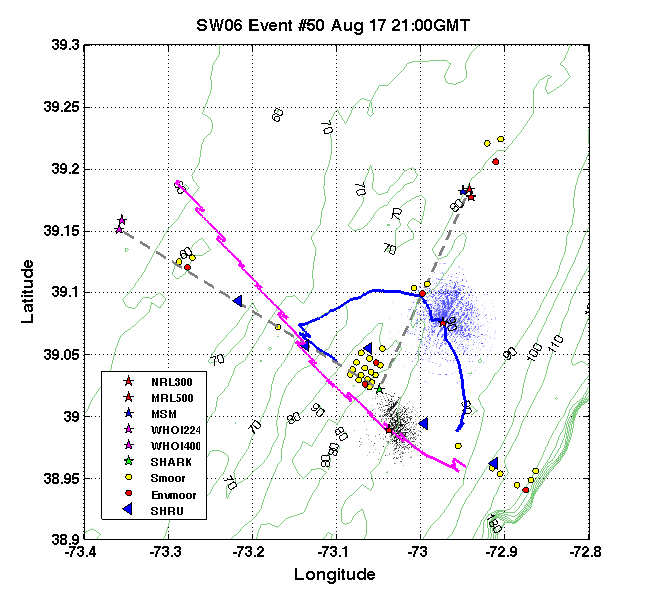
\includegraphics[width=\textwidth]{Aug17_2100_t.png}
  \caption{Surface expression of internal wave package at 21:00GMT, Aug. 17, recorded by R/V Sharp and R/V Oceanus. Blue and red lines indicate their movements, respectively. (Blue: R/V Sharp's, red: R/V Oceanus'}\label{fig:r2130_r}
\end{figure}

\begin{figure}[H]
  \centering
  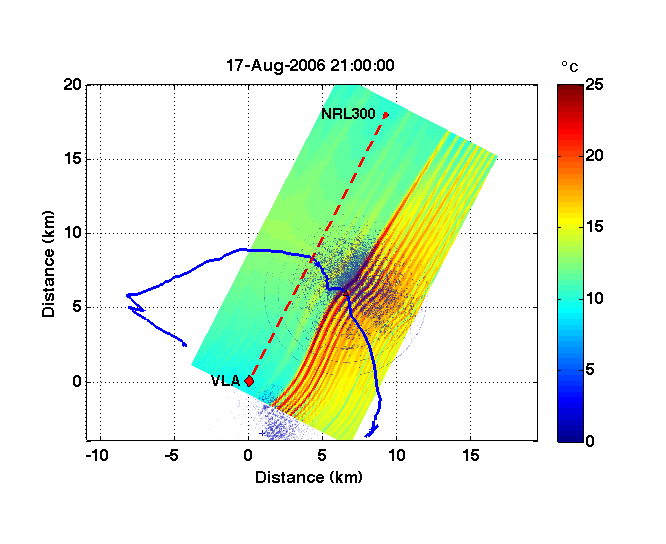
\includegraphics[width=\textwidth]{sw06_Tempr_Depth30m_2006Aug17_210000_radar_curve_thesis1.png}
  \caption{Interpolated internal wave field at 21:00GMT, Aug. 17, water depth = 20m. (Refer to section 3.4 for detailed interpolation method)}\label{fig:r2130_i}
\end{figure}

\begin{figure}[H]
  \centering
  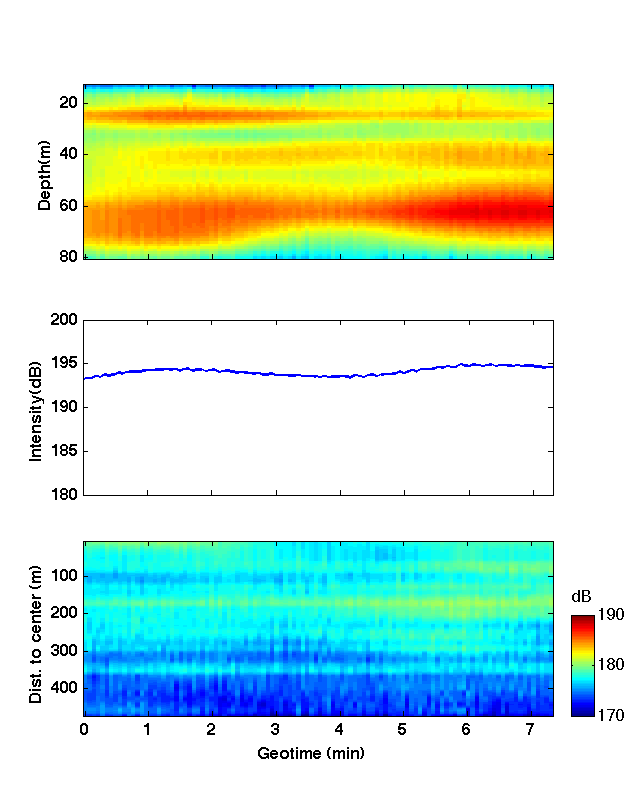
\includegraphics[width=\textwidth]{nrl300_060817T2100_vla_hla_intens_geotime2.png}
  \caption{Received signal on Shark VLA (top), HLA (bottom) and signal intensity (middle) from Aug.17 21:00GMT to 21:07GMT }\label{fig:a2130}
\end{figure}

\begin{figure}[H]
  \centering
  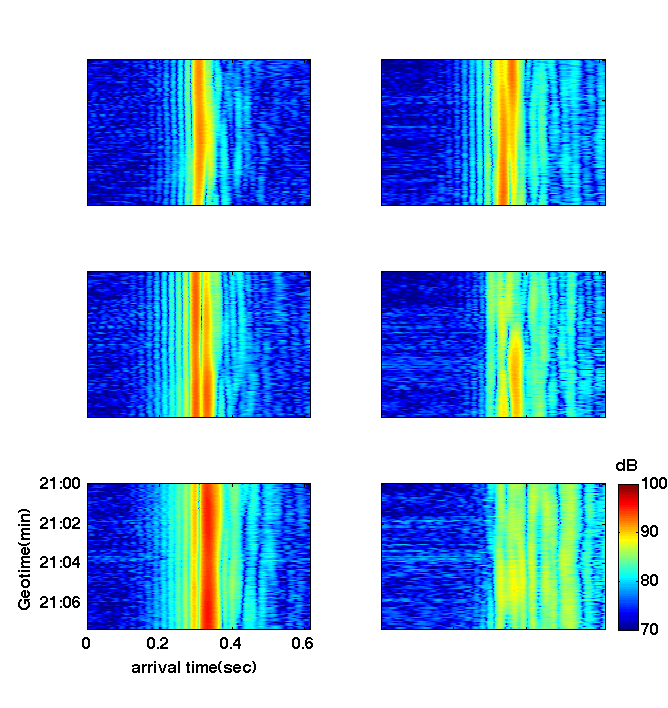
\includegraphics[width=\textwidth]{sw06_broadband_mf_nrl300_F2_6in1_thesis.png}
  \caption{Mode decomposition of received signal on Shark VLA. 
    Left column: mode 1-3, right column: mode 4-6 }\label{fig:m2130}
\end{figure}


%--F3
\begin{figure}[H]
  \centering
  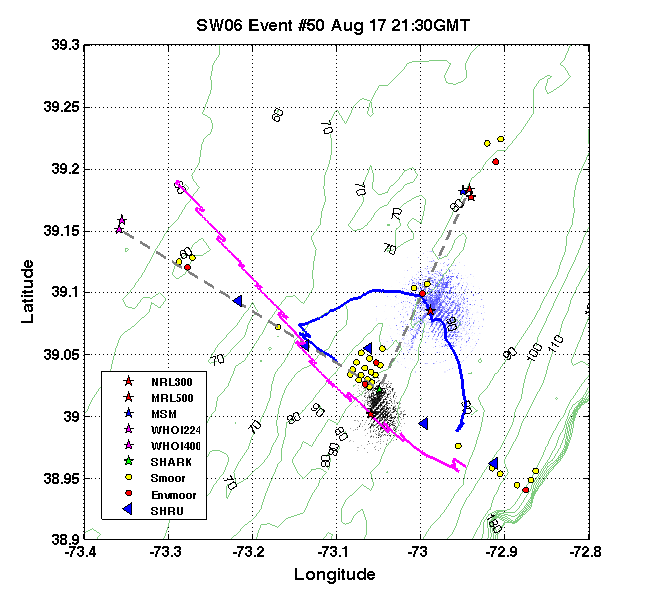
\includegraphics[width=\textwidth]{Aug17_2130_t.png}
  \caption{Surface expression of internal wave package at 21:30GMT, Aug. 17, recorded by R/V Sharp and R/V Oceanus. Blue and red lines indicate their movements, respectively. (Blue: R/V Sharp's, red: R/V Oceanus'}\label{fig:r2130_r}
\end{figure}

\begin{figure}[H]
  \centering
  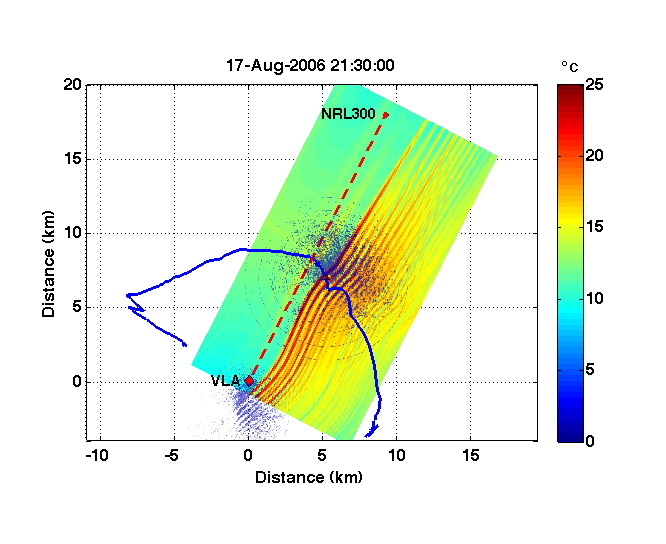
\includegraphics[width=\textwidth]{sw06_Tempr_Depth30m_2006Aug17_213000_radar_curve_thesis1.png}
  \caption{Interpolated internal wave field at 21:30GMT, Aug. 17, water depth = 20m. (Refer to section 3.4 for detailed interpolation method)}\label{fig:r2130_i}
\end{figure}

\begin{figure}[H]
  \centering
  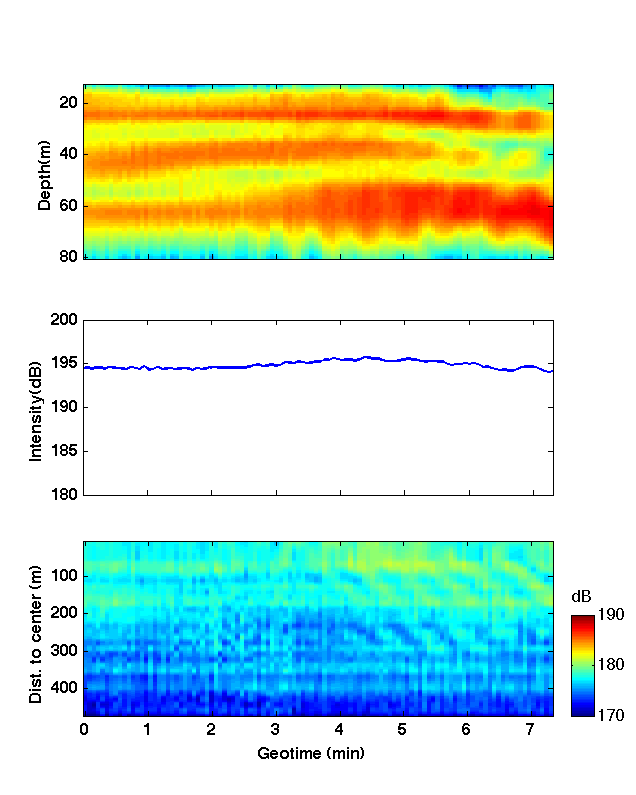
\includegraphics[width=\textwidth]{nrl300_060817T2130_vla_hla_intens_geotime2.png}
  \caption{Received signal on Shark VLA (top), HLA (bottom) and signal intensity (middle) from Aug.17 21:30GMT to 21:37GMT }\label{fig:a2130}
\end{figure}

\begin{figure}[H]
  \centering
  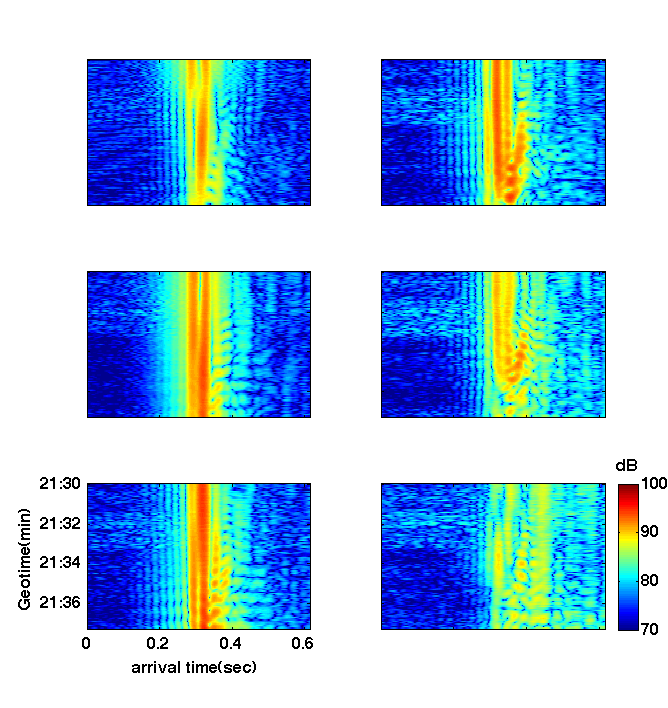
\includegraphics[width=\textwidth]{sw06_broadband_mf_nrl300_F3_6in1_thesis.png}
  \caption{Mode decomposition of received signal on Shark VLA. 
    Left column: mode 1-3, right column: mode 4-6 }\label{fig:m2130}
\end{figure}
\clearpage

%%--F4
\begin{figure}[H]
  \centering
  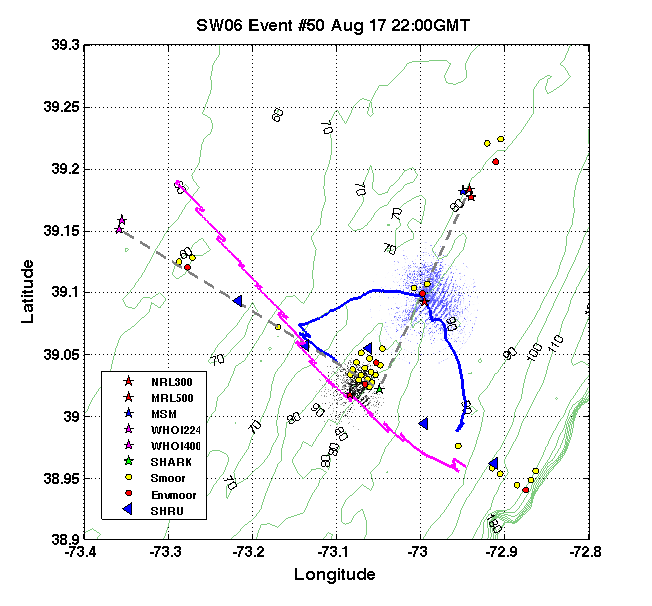
\includegraphics[width=\textwidth]{Aug17_2200_t.png}
  \caption{Surface expression of internal wave package at 22:00GMT, Aug. 17, recorded by R/V Sharp and R/V Oceanus. Blue and red lines indicate their movements, respectively. (Blue: R/V Sharp's, red: R/V Oceanus'}\label{fig:r2130_r}
\end{figure}

\begin{figure}[H]
  \centering
  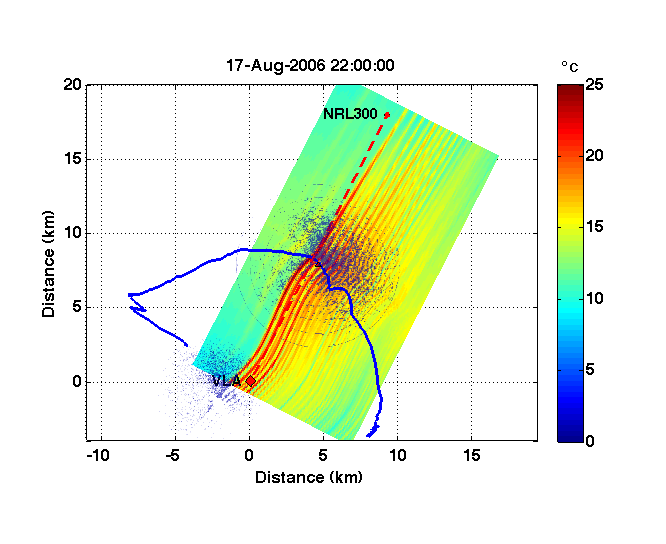
\includegraphics[width=\textwidth]{sw06_Tempr_Depth30m_2006Aug17_220000_radar_curve_thesis1.png}
  \caption{Interpolated internal wave field at 22:00GMT, Aug. 17, water depth = 20m. (Refer to section 3.4 for detailed interpolation method)}\label{fig:r2130_i}
\end{figure}

\begin{figure}[H]
  \centering
  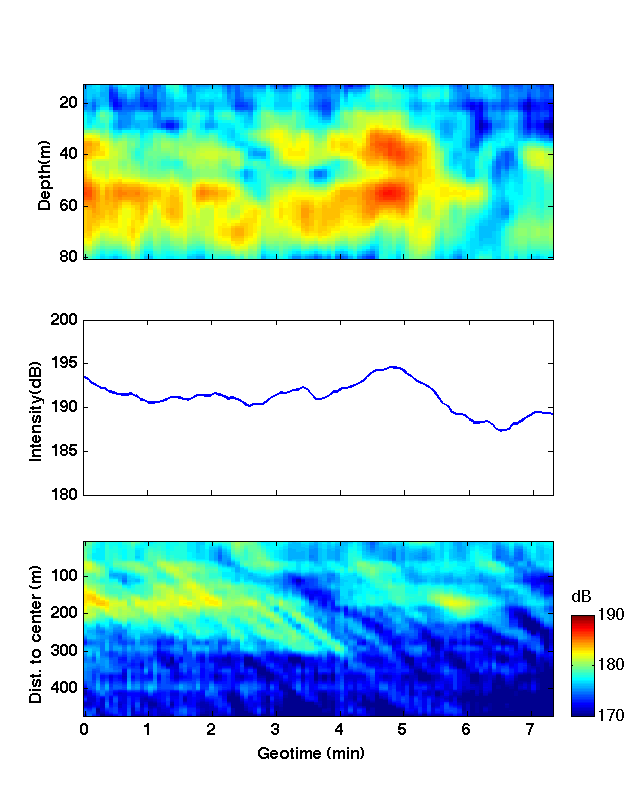
\includegraphics[width=\textwidth]{nrl300_060817T2200_vla_hla_intens_geotime2.png}
  \caption{Received signal on Shark VLA (top), HLA (bottom) and signal intensity (middle) from Aug.17 22:00GMT to 22:07GMT }\label{fig:a2130}
\end{figure}

\begin{figure}[H]
  \centering
  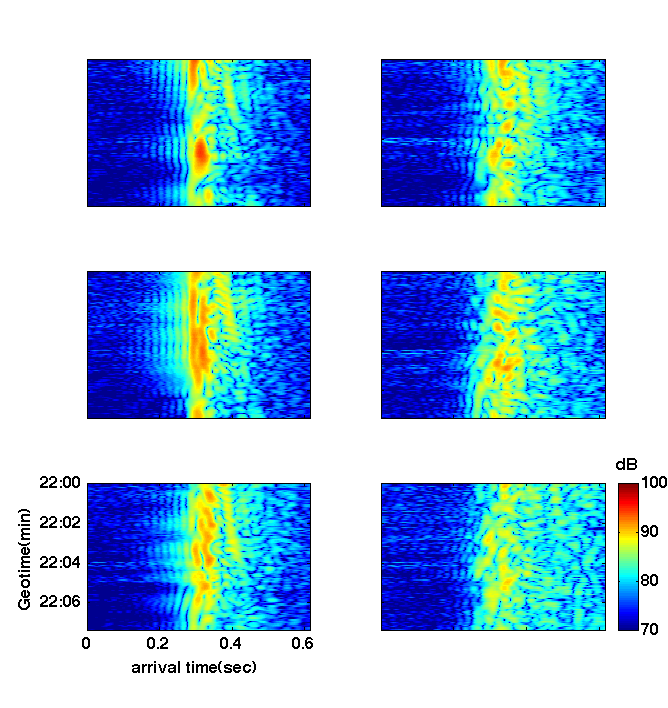
\includegraphics[width=\textwidth]{sw06_broadband_mf_nrl300_F4_6in1_thesis.png}
  \caption{Mode decomposition of received signal on Shark VLA. 
    Left column: mode 1-3, right column: mode 4-6 }\label{fig:m2130}
\end{figure}


%%--F5
\begin{figure}[H]
  \centering
  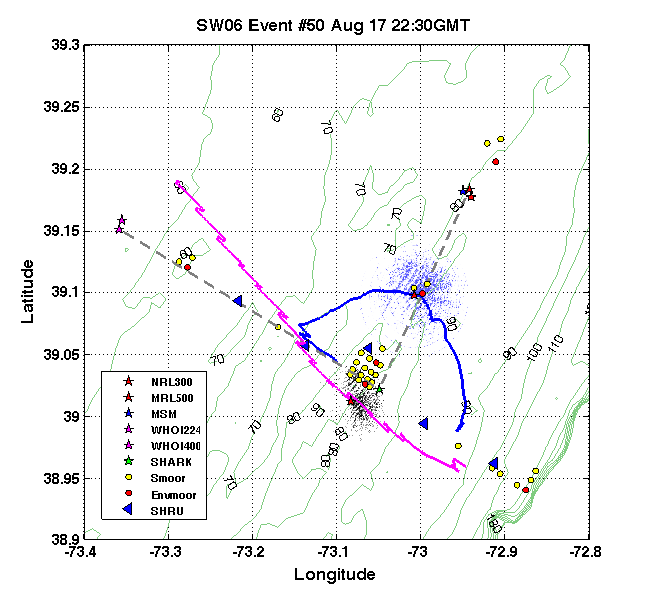
\includegraphics[width=\textwidth]{Aug17_2230_t.png}
  \caption{Surface expression of internal wave package at 22:30GMT, Aug. 17, recorded by R/V Sharp and R/V Oceanus. Blue and red lines indicate their movements, respectively. (Blue: R/V Sharp's, red: R/V Oceanus'}\label{fig:r2130_r}
\end{figure}

\begin{figure}[H]
 \centering
 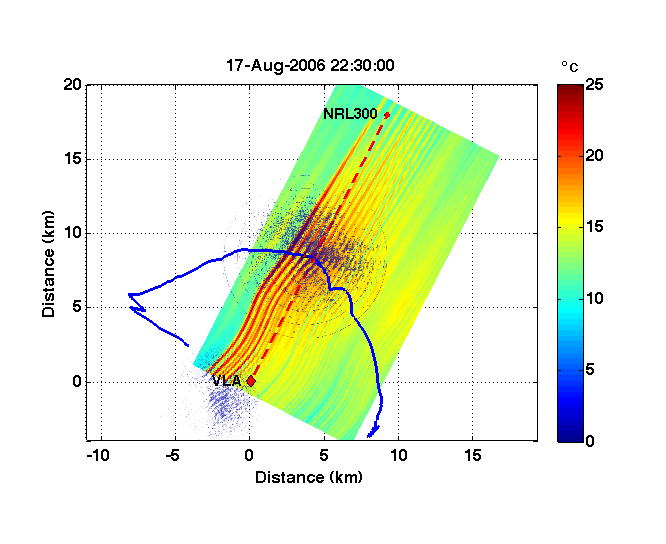
\includegraphics[width=\textwidth]{sw06_Tempr_Depth30m_2006Aug17_223000_radar_curve_thesis1.png}
 \caption{Interpolated internal wave field at 22:30GMT, Aug. 17, water depth = 20m. (Refer to section 3.4 for detailed interpolation method)}\label{fig:r2130_i}
\end{figure}

\begin{figure}[H]
  \centering
  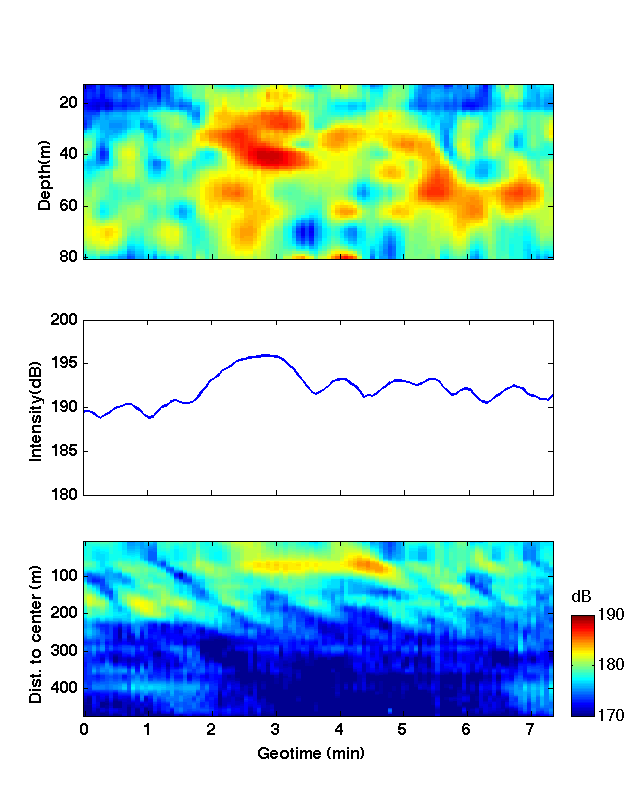
\includegraphics[width=\textwidth]{nrl300_060817T2230_vla_hla_intens_geotime2.png}
  \caption{Received signal on Shark VLA (top), HLA (bottom) and signal intensity (middle) from Aug.17 22:30GMT to 22:37GMT }\label{fig:a2130}
\end{figure}

\begin{figure}[h]
\centering
 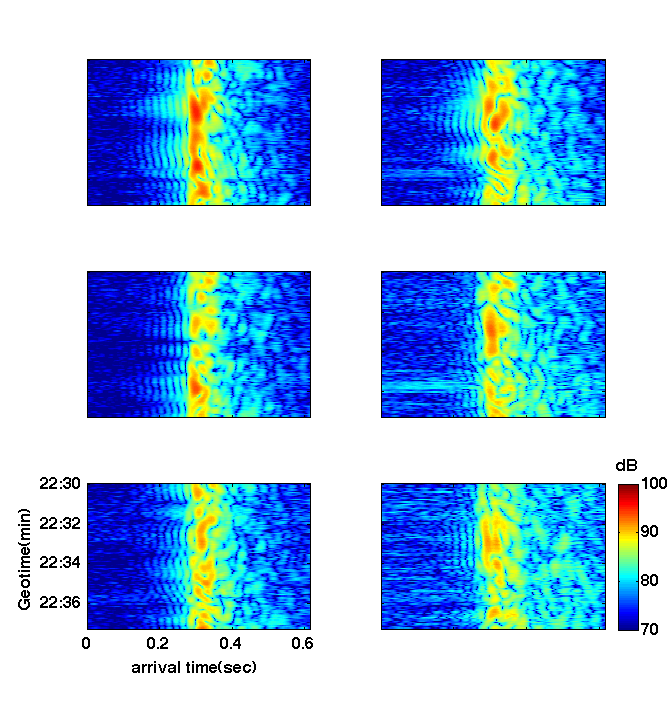
\includegraphics[width=\textwidth]{sw06_broadband_mf_nrl300_F5_6in1_thesis.png}
  \caption{Mode decomposition of received signal on Shark VLA. 
    Left column: mode 1-3, right column: mode 4-6 }\label{fig:m2130}
\end{figure}


%%--M1
\begin{figure}[H]
  \centering
  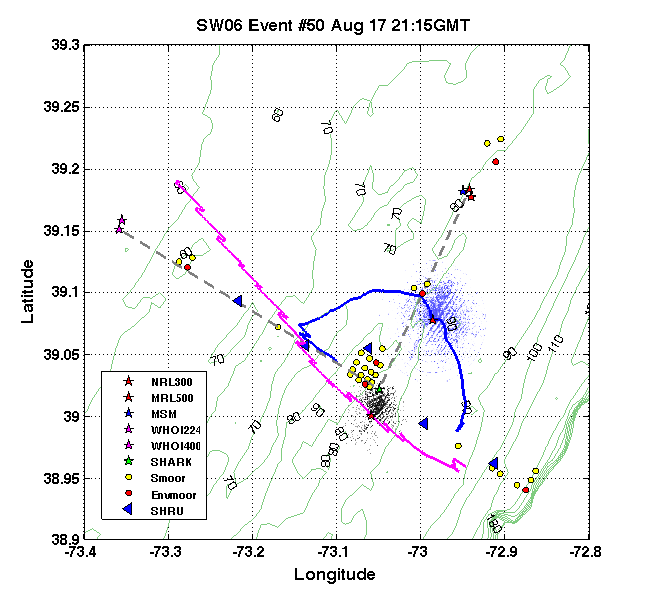
\includegraphics[width=\textwidth]{Aug17_2115_t.png}
  \caption{Surface expression of internal wave package at 21:15GMT, Aug. 17, recorded by R/V Sharp and R/V Oceanus. Blue and red lines indicate their movements, respectively. (Blue: R/V Sharp's, red: R/V Oceanus'}\label{fig:r2130_r}
\end{figure}

%\begin{figure}[H]
% \centering
% 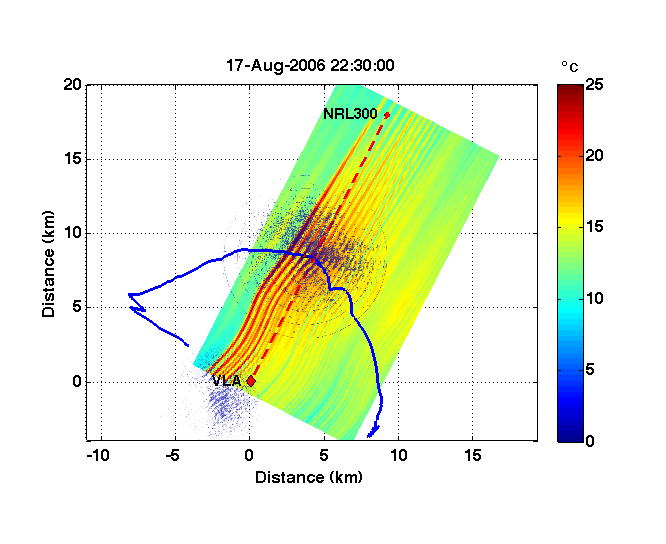
\includegraphics[width=\textwidth]{sw06_Tempr_Depth30m_2006Aug17_223000_radar_curve_thesis1.png}
% \caption{Interpolated internal wave field at 22:30GMT, Aug. 17, water depth = 20m. (Refer to section 3.4 for detailed interpolation method)}\label{fig:r2130_i}
%\end{figure}

\begin{figure}[H]
  \centering
  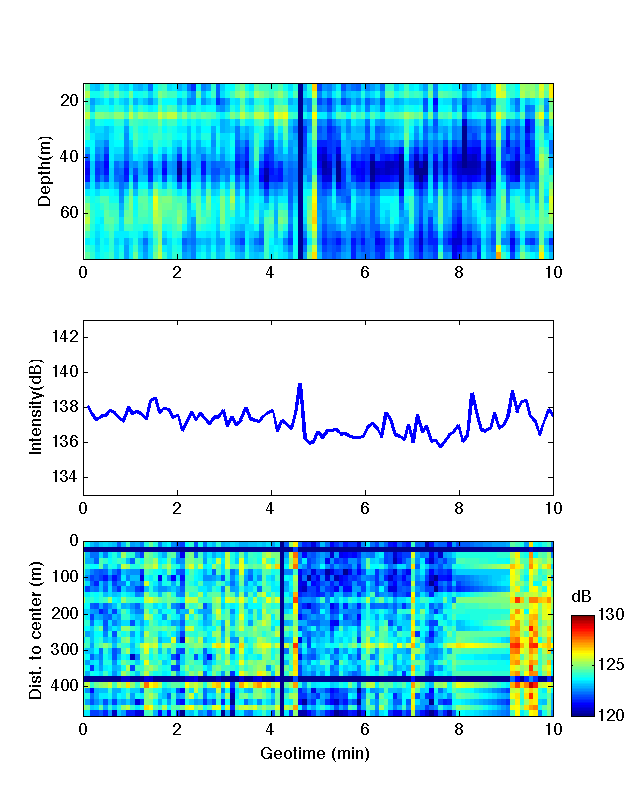
\includegraphics[width=\textwidth]{udel_060817T2115_vla_hla_intens_geotime2.png}
  \caption{Received signal on Shark VLA (top), HLA (bottom) and signal intensity (middle) from Aug.17 21:15GMT to 21:25GMT }\label{fig:a2130}
\end{figure}

%\begin{figure}[h]
%\centering
% 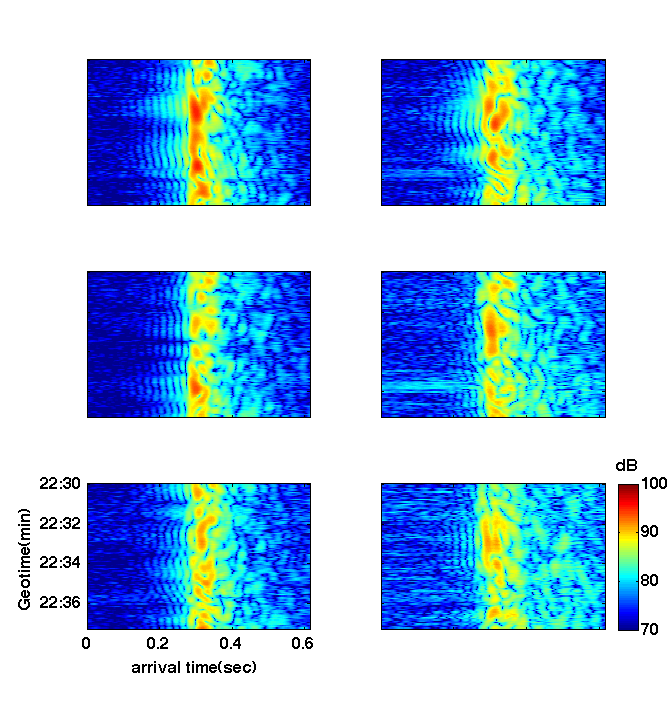
\includegraphics[width=\textwidth]{sw06_broadband_mf_nrl300_F5_6in1_thesis.png}
%  \caption{Mode decomposition of received signal on Shark VLA. 
 %   Left column: mode 1-3, right column: mode 4-6 }\label{fig:m2130}
%\end{figure}


%%--M2
\begin{figure}[H]
  \centering
  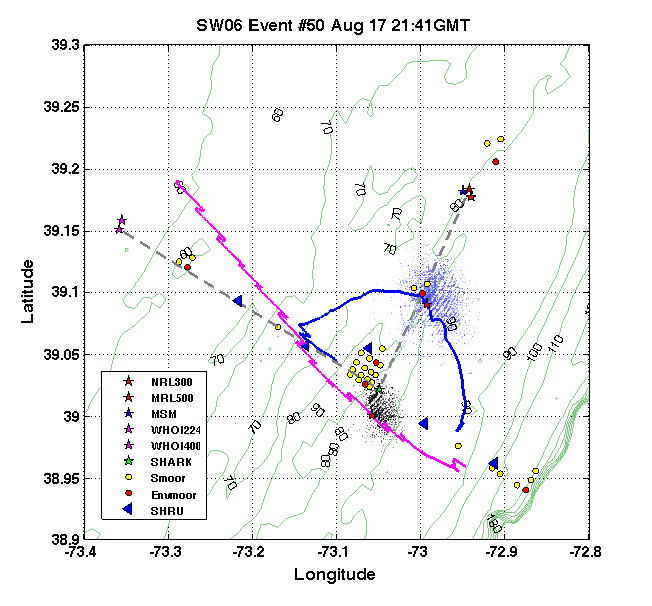
\includegraphics[width=\textwidth]{Aug17_2141_t.png}
  \caption{Surface expression of internal wave package at 21:41GMT, Aug. 17, recorded by R/V Sharp and R/V Oceanus. Blue and red lines indicate their movements, respectively. (Blue: R/V Sharp's, red: R/V Oceanus'}\label{fig:r2130_r}
\end{figure}

%\begin{figure}[H]
% \centering
% 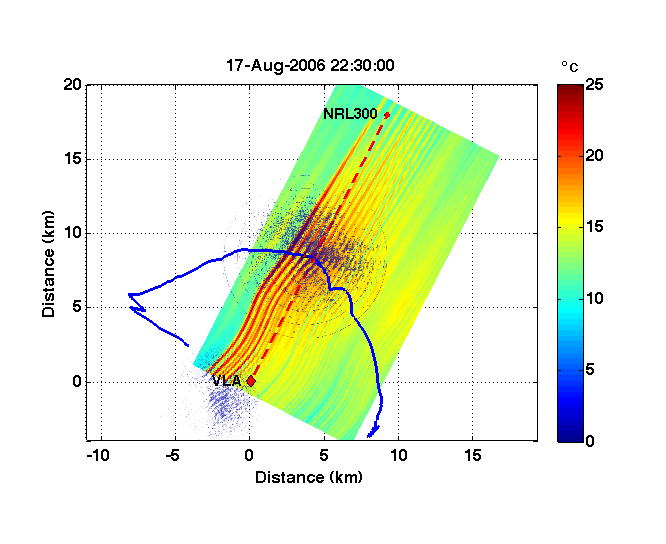
\includegraphics[width=\textwidth]{sw06_Tempr_Depth30m_2006Aug17_223000_radar_curve_thesis1.png}
% \caption{Interpolated internal wave field at 22:30GMT, Aug. 17, water depth = 20m. (Refer to section 3.4 for detailed interpolation method)}\label{fig:r2130_i}
%\end{figure}

\begin{figure}[H]
  \centering
  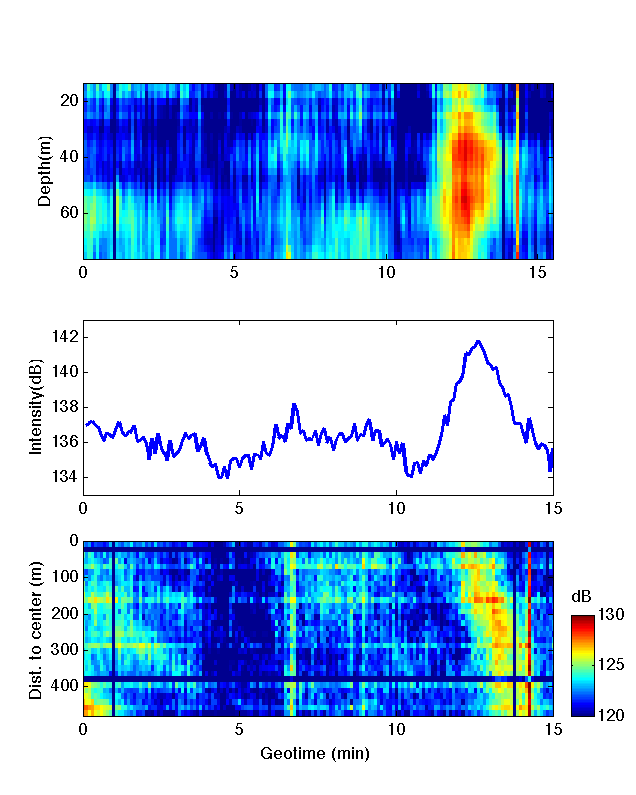
\includegraphics[width=\textwidth]{udel_060817T2141_vla_hla_intens_geotime2.png}
  \caption{Received signal on Shark VLA (top), HLA (bottom) and signal intensity (middle) from Aug.17 21:41GMT to 21:56GMT }\label{fig:a2130}
\end{figure}

%\begin{figure}[h]
%\centering
% 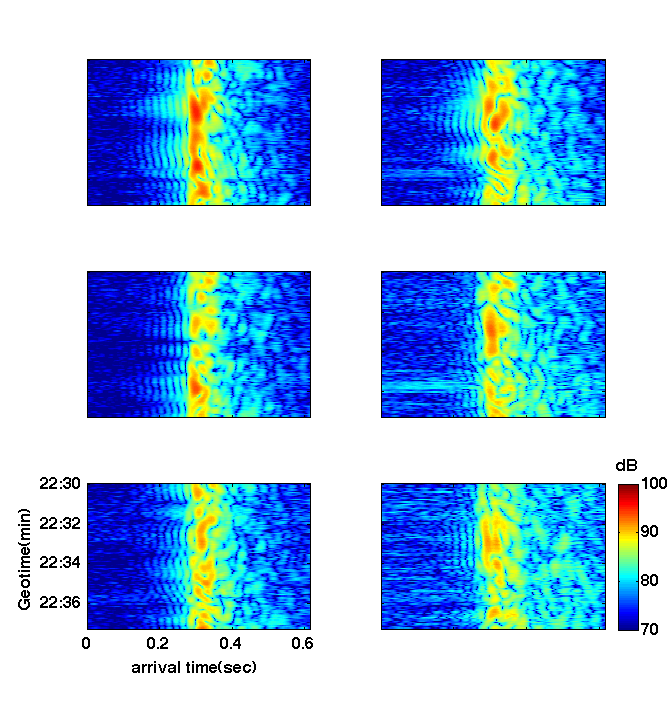
\includegraphics[width=\textwidth]{sw06_broadband_mf_nrl300_F5_6in1_thesis.png}
%  \caption{Mode decomposition of received signal on Shark VLA. 
 %   Left column: mode 1-3, right column: mode 4-6 }\label{fig:m2130}
%\end{figure}


%%--M3
\begin{figure}[H]
  \centering
  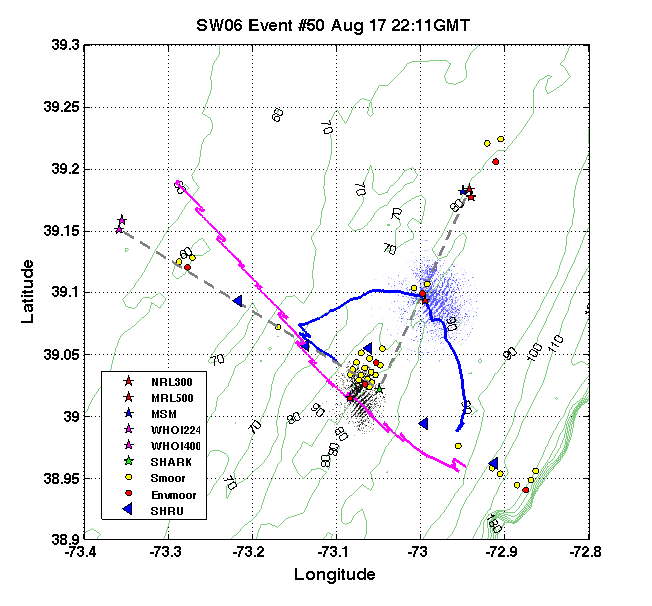
\includegraphics[width=\textwidth]{Aug17_2211_t.png}
  \caption{Surface expression of internal wave package at 22:11GMT, Aug. 17, recorded by R/V Sharp and R/V Oceanus. Blue and red lines indicate their movements, respectively. (Blue: R/V Sharp's, red: R/V Oceanus'}\label{fig:r2130_r}
\end{figure}

%\begin{figure}[H]
% \centering
% 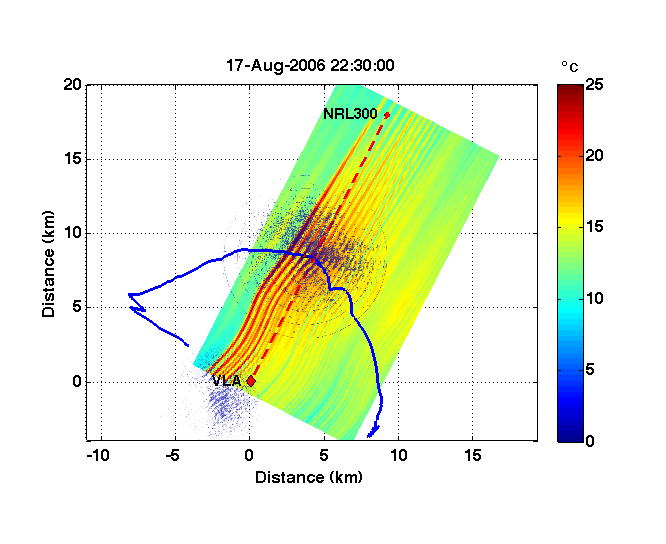
\includegraphics[width=\textwidth]{sw06_Tempr_Depth30m_2006Aug17_223000_radar_curve_thesis1.png}
% \caption{Interpolated internal wave field at 22:30GMT, Aug. 17, water depth = 20m. (Refer to section 3.4 for detailed interpolation method)}\label{fig:r2130_i}
%\end{figure}

\begin{figure}[H]
  \centering
  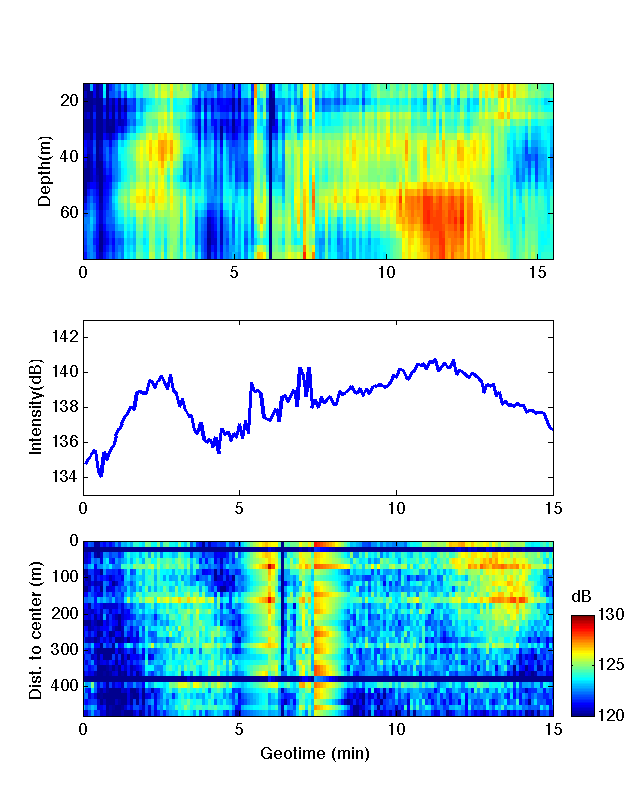
\includegraphics[width=\textwidth]{udel_060817T2211_vla_hla_intens_geotime2.png}
  \caption{Received signal on Shark VLA (top), HLA (bottom) and signal intensity (middle) from Aug.17 22:11GMT to 22:26GMT }\label{fig:a2130}
\end{figure}

%\begin{figure}[h]
%\centering
% 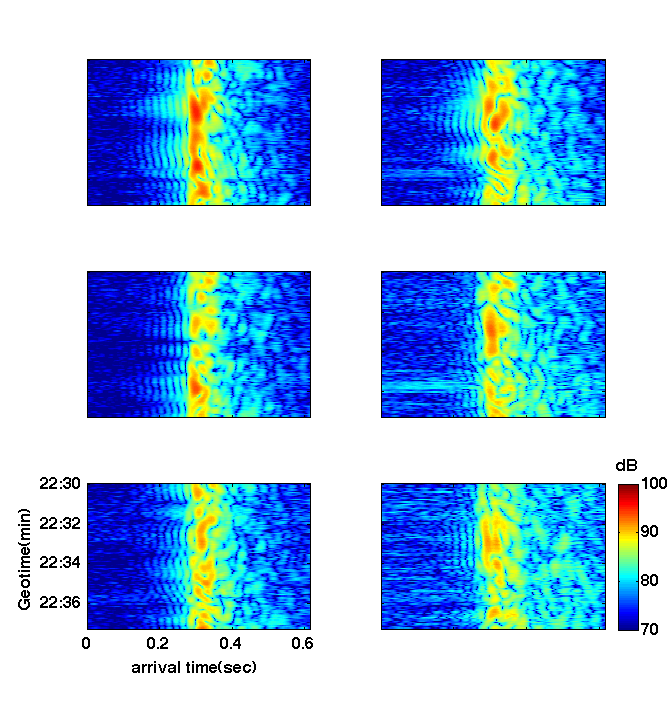
\includegraphics[width=\textwidth]{sw06_broadband_mf_nrl300_F5_6in1_thesis.png}
%  \caption{Mode decomposition of received signal on Shark VLA. 
 %   Left column: mode 1-3, right column: mode 4-6 }\label{fig:m2130}
%\end{figure}


%%--M4
\begin{figure}[H]
  \centering
  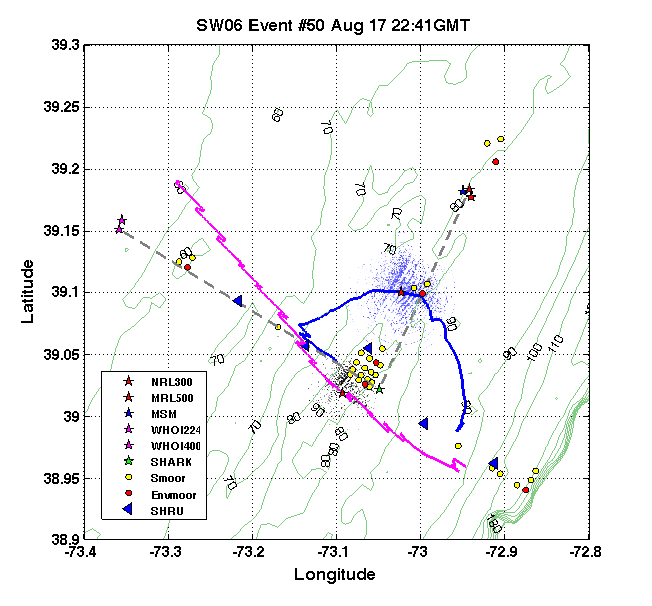
\includegraphics[width=\textwidth]{Aug17_2241_t.png}
  \caption{Surface expression of internal wave package at 22:41GMT, Aug. 17, recorded by R/V Sharp and R/V Oceanus. Blue and red lines indicate their movements, respectively. (Blue: R/V Sharp's, red: R/V Oceanus'}\label{fig:r2130_r}
\end{figure}

%\begin{figure}[H]
% \centering
% 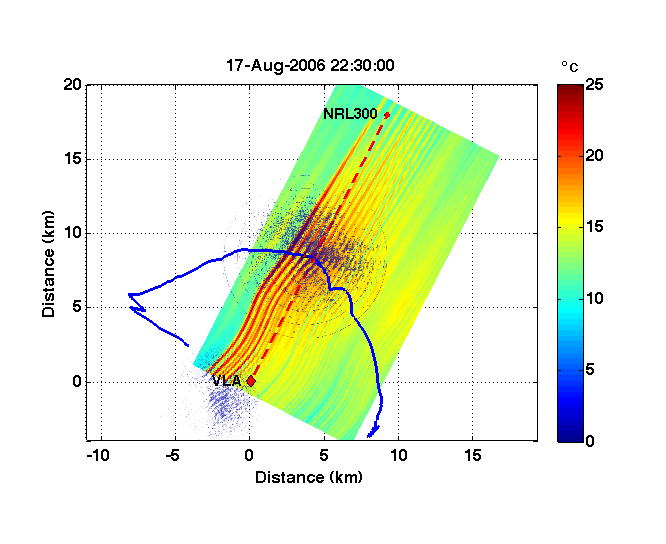
\includegraphics[width=\textwidth]{sw06_Tempr_Depth30m_2006Aug17_223000_radar_curve_thesis1.png}
% \caption{Interpolated internal wave field at 22:30GMT, Aug. 17, water depth = 20m. (Refer to section 3.4 for detailed interpolation method)}\label{fig:r2130_i}
%\end{figure}

\begin{figure}[H]
  \centering
  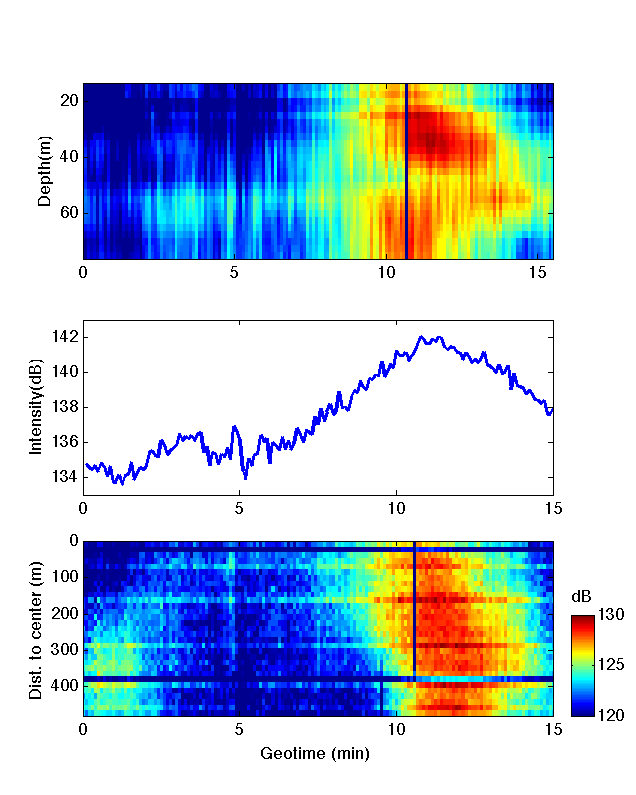
\includegraphics[width=\textwidth]{udel_060817T2241_vla_hla_intens_geotime2.png}
  \caption{Received signal on Shark VLA (top), HLA (bottom) and signal intensity (middle) from Aug.17 22:41GMT to 22:46GMT }\label{fig:a2130}
\end{figure}

%\begin{figure}[h]
%\centering
% 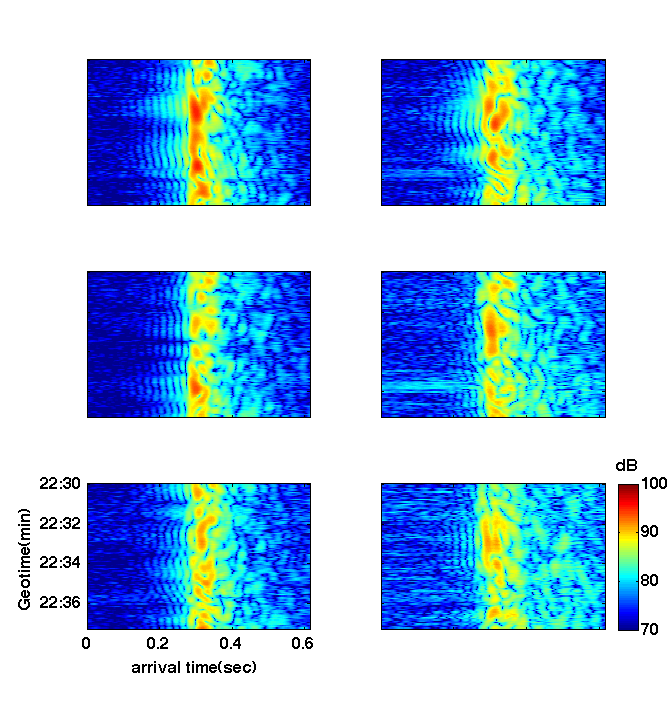
\includegraphics[width=\textwidth]{sw06_broadband_mf_nrl300_F5_6in1_thesis.png}
%  \caption{Mode decomposition of received signal on Shark VLA. 
 %   Left column: mode 1-3, right column: mode 4-6 }\label{fig:m2130}
%\end{figure}


%%--M5
\begin{figure}[H]
  \centering
  \includegraphics[width=\textwidth]{Aug17_2311_t.png}
  \caption{Surface expression of internal wave package at 23:11GMT, Aug. 17, recorded by R/V Sharp and R/V Oceanus. Blue and red lines indicate their movements, respectively. (Blue: R/V Sharp's, red: R/V Oceanus'}\label{fig:r2130_r}
\end{figure}

%\begin{figure}[H]
% \centering
% \includegraphics[width=\textwidth]{sw06_Tempr_Depth30m_2006Aug17_223000_radar_curve_thesis1.png}
% \caption{Interpolated internal wave field at 22:30GMT, Aug. 17, water depth = 20m. (Refer to section 3.4 for detailed interpolation method)}\label{fig:r2130_i}
%\end{figure}

\begin{figure}[H]
  \centering
  \includegraphics[width=\textwidth]{udel_060817T2311_vla_hla_intens_geotime2.png}
  \caption{Received signal on Shark VLA (top), HLA (bottom) and signal intensity (middle) from Aug.17 23:11GMT to 23:26GMT }\label{fig:a2130}
\end{figure}



\clearpage


\begin{figure}[H]
  \centering
  \includegraphics[width=0.6\textwidth]{angular_distr_4.png}
  \caption{Data of depth-integrated intensity and estimated angle for each zone }\label{fig:a2130}
\end{figure}

%%CHAP. Analysis


\begin{figure}[H]
  \centering
  \includegraphics[width=0.8\textwidth]{kraken_results.png}
  \caption{From left to right, vertical modes 1-4 excited by a 330Hz frequency signal. Temperature data were recorded at NRL300 source, GMT21:30, Aug 17, 2006.}\label{fig:a2130}
\end{figure}


\begin{figure}[H]
  \centering
  \includegraphics[width=\textwidth]{mode_6in1_ll_paper_small.png}
  \caption{Broadband model decomposition of acoustic signal from 21:30GMT to 21:37GMT (mode1-6).}\label{fig:a2130}
\end{figure}

\begin{figure}[H]
  \centering
  \includegraphics[width=\textwidth]{MC_213000_m_all_copy.png}
  \caption{PE modal coupling. From left to right, the excited modes at source; from top to bottom, the coupled modes. Most energy is confined at the excited mode at the source, which is consistent with the theory about adiabatic propagation at near-parallel environment.  Higher modes show stronger coupling effects than lower modes. Energy from mode 1 will couple to mode 3, while mode 4 can couple up to mode 8. }\label{fig:a2130}
\end{figure}


\begin{figure}[H]
  \centering
  \includegraphics[width=\textwidth]{sw06_event50_PE_NRL300_300Hz_17Aug06_213000_MC_m1_3_copy_small.png}
  \caption{(Modal dependence) Acoustic intensity is shown for vertical modes 1~3 at GMT21:30:00(left) and GMT 21:43:40(right) respectively.  A single frequency signal (330Hz) source is placed at (0,0), depth = 70m. Temperature contour overlay shows the passing internal waves. }\label{fig:a2130}
\end{figure}


\begin{figure}[H]
  \centering
  \includegraphics[width=\textwidth]{270_330_M1_3_213000_small.png}
  \caption{(Frequency dependence) Acoustic integrated sound intensity of vertical modes 1-3 at frequency = 270Hz, 330Hz at GMT21:30:00. Source position (x,y) = (0, 0) and source depth = 70m. Temperature contour overlay shows the passing internal waves. }\label{fig:a2130}
\end{figure}



\begin{figure}[H]
  \centering
  \includegraphics[width=\textwidth]{moving_pe.jpg}
  \caption{3-D PE modeling results showing the acoustic intensity and the temperature contour at depth 20 m.  Source is located at point (0,0) and white dashed lines indicate the acoustic track. }\label{fig:a2130}
\end{figure}

\begin{figure}[H]
  \centering
  \includegraphics[width=\textwidth]{M3_comparison.jpg}
  \caption{(a) Data and (b) model comparison of the intensity as a function of depth (top panels) and depth-integrated intensity (bottom panels) on Zone 3, August 17, 2006 at 22:11 to 22:26 GMT.  The occurrence of focusing at geotime about 22:21:30 observed in the data was well predicted by the model.}\label{fig:a2130}
\end{figure}


\begin{figure}[H]
  \centering
  \includegraphics[width=1.2\textwidth,angle=90]{sw06_udel_pe_exp_comparison.png}
  \caption{PE model results and experiment data comparison for moving source J15. Solid line shows the results of 3D PE model. The propagating angles are shown at the top for the beginning and end of each transmission session}\label{fig:a2130}
\end{figure}

